%%
%% midwife.tex — Project report for CSC2524 (Human-Centred AI), Winter 2026
%% Uses the ACM sigconf authordraft template.
%%
%% Compile with: pdflatex midwife && bibtex midwife && pdflatex midwife && pdflatex midwife
%%
\documentclass[sigconf,authordraft]{acmart}

%% ── Metadata ──────────────────────────────────────────────────────────────────
\setcopyright{none}
\copyrightyear{2026}
\acmYear{2026}
\acmDOI{}
\acmConference[CSC2524 '26]{CSC2524: Topics in Interactive Computing — Human-Centred AI}{March 30, 2026}{Toronto, ON, Canada}
\acmISBN{}

%% ── Document ──────────────────────────────────────────────────────────────────
\begin{document}

\title{midWife: Enabling Open-Ended Planning via Socratic Dialogue with Large Language Models}

\author{Aditya Shukla}
\email{adshukla@cs.toronto.edu}
\affiliation{%
  \department{Department of Computer Science}
  \institution{University of Toronto}
  \city{Toronto}
  \state{Ontario}
  \country{Canada}
}

\renewcommand{\shortauthors}{Shukla}

%% ── Abstract ──────────────────────────────────────────────────────────────────
\begin{abstract}
%%
%% TARGET: ~150 words.
%%
%% Cover all four beats in order:
%%   (1) The problem: LLM chat interfaces are one-dimensional; they cannot
%%       represent the branching, multi-dimensional structure of real planning.
%%   (2) The approach: MidWife models planning as a Socratic discourse tree —
%%       a hierarchical structure of Aspects (clarifying questions) that the user
%%       navigates and answers in partnership with an LLM.
%%   (3) Key features worth naming: 9 planning modes, per-node chat assistant,
%%       ghost-node prefetching, ancestor recontextualization, synthesis panel.
%%   (4) Contribution: a working prototype + design insights toward AI as a
%%       Socratic thinking partner in structured planning interfaces.
%%
Large Language Models (LLMs) have enabled users to engage in planning, reasoning
and sensemaking with a ``thought partner'' of sorts, allowing open-ended discussions
on nuanced subjects. This mirrors the idea of a \textit{Socratic interlocutor}
asking probing questions --- serving to help users formalize their thinking, flesh
out new ideas, and even find holes in their planning. However, most LLM platforms
are limited to one-dimensional chat interfaces that cannot adjust to the scope of a
dynamic, ever-growing discourse, thereby limiting the ability of a user to build a
map of their thinking. This reflects an inherent limitation in the affordances offered
by a linear conversational interface. We present \textbf{\textit{midWife}}: an interactive
system that encourages thinking by iteratively soliciting the user's intent, objective
and/or nascent thoughts, probing with revelatory questions to concretize
user-indicated notions, and visualizing this discourse as a map of thinking in the
form of a node-link diagram connecting a central Thesis with its many Aspects. At
each iteration, the user may (i)~solicit more probing questions conditioned on a
specific Aspect (if they are unsure of what to explore next); or (ii)~manually add
one or more Aspects at any point of the map (if they already know what to explore).
Parallelly, a Plan is generated by midWife in rich Markdown, updated incrementally
to reflect the growing map of thinking. A persistent chat interface allows users to
ask questions, request changes, and steer the Plan toward their focus areas.
\end{abstract}

%% ── CCS Concepts ──────────────────────────────────────────────────────────────
%% Generate the authoritative XML+commands from: https://dl.acm.org/ccs/ccs.cfm
%% Suggested concepts:
%%   Human-centered computing → HCI → Interactive systems and tools  [500]
%%   Human-centered computing → HCI → Natural language interfaces    [300]
%%   Computing methodologies  → AI  → Natural language processing     [100]
\begin{CCSXML}
<ccs2012>
 <concept>
  <concept_id>10003120.10003121.10003128</concept_id>
  <concept_desc>Human-centered computing~Interactive systems and tools</concept_desc>
  <concept_significance>500</concept_significance>
 </concept>
 <concept>
  <concept_id>10003120.10003121.10003124.10010870</concept_id>
  <concept_desc>Human-centered computing~Natural language interfaces</concept_desc>
  <concept_significance>300</concept_significance>
 </concept>
 <concept>
  <concept_id>10010147.10010178.10010187</concept_id>
  <concept_desc>Computing methodologies~Natural language processing</concept_desc>
  <concept_significance>100</concept_significance>
 </concept>
</ccs2012>
\end{CCSXML}

\ccsdesc[500]{Human-centered computing~Interactive systems and tools}
\ccsdesc[300]{Human-centered computing~Natural language interfaces}
\ccsdesc[100]{Computing methodologies~Natural language processing}

\keywords{Socratic dialogue, discourse trees, structured thinking, LLM-assisted planning, mixed-initiative interaction, sensemaking}

%% ── Teaser Figure ─────────────────────────────────────────────────────────────
%% Use a full-width screenshot of the discourse canvas — ideally a real session
%% showing a thesis node, several answered aspect nodes, an open chat panel,
%% and the synthesis panel on the right. Place the image at figures/teaser.png.
\begin{teaserfigure}
  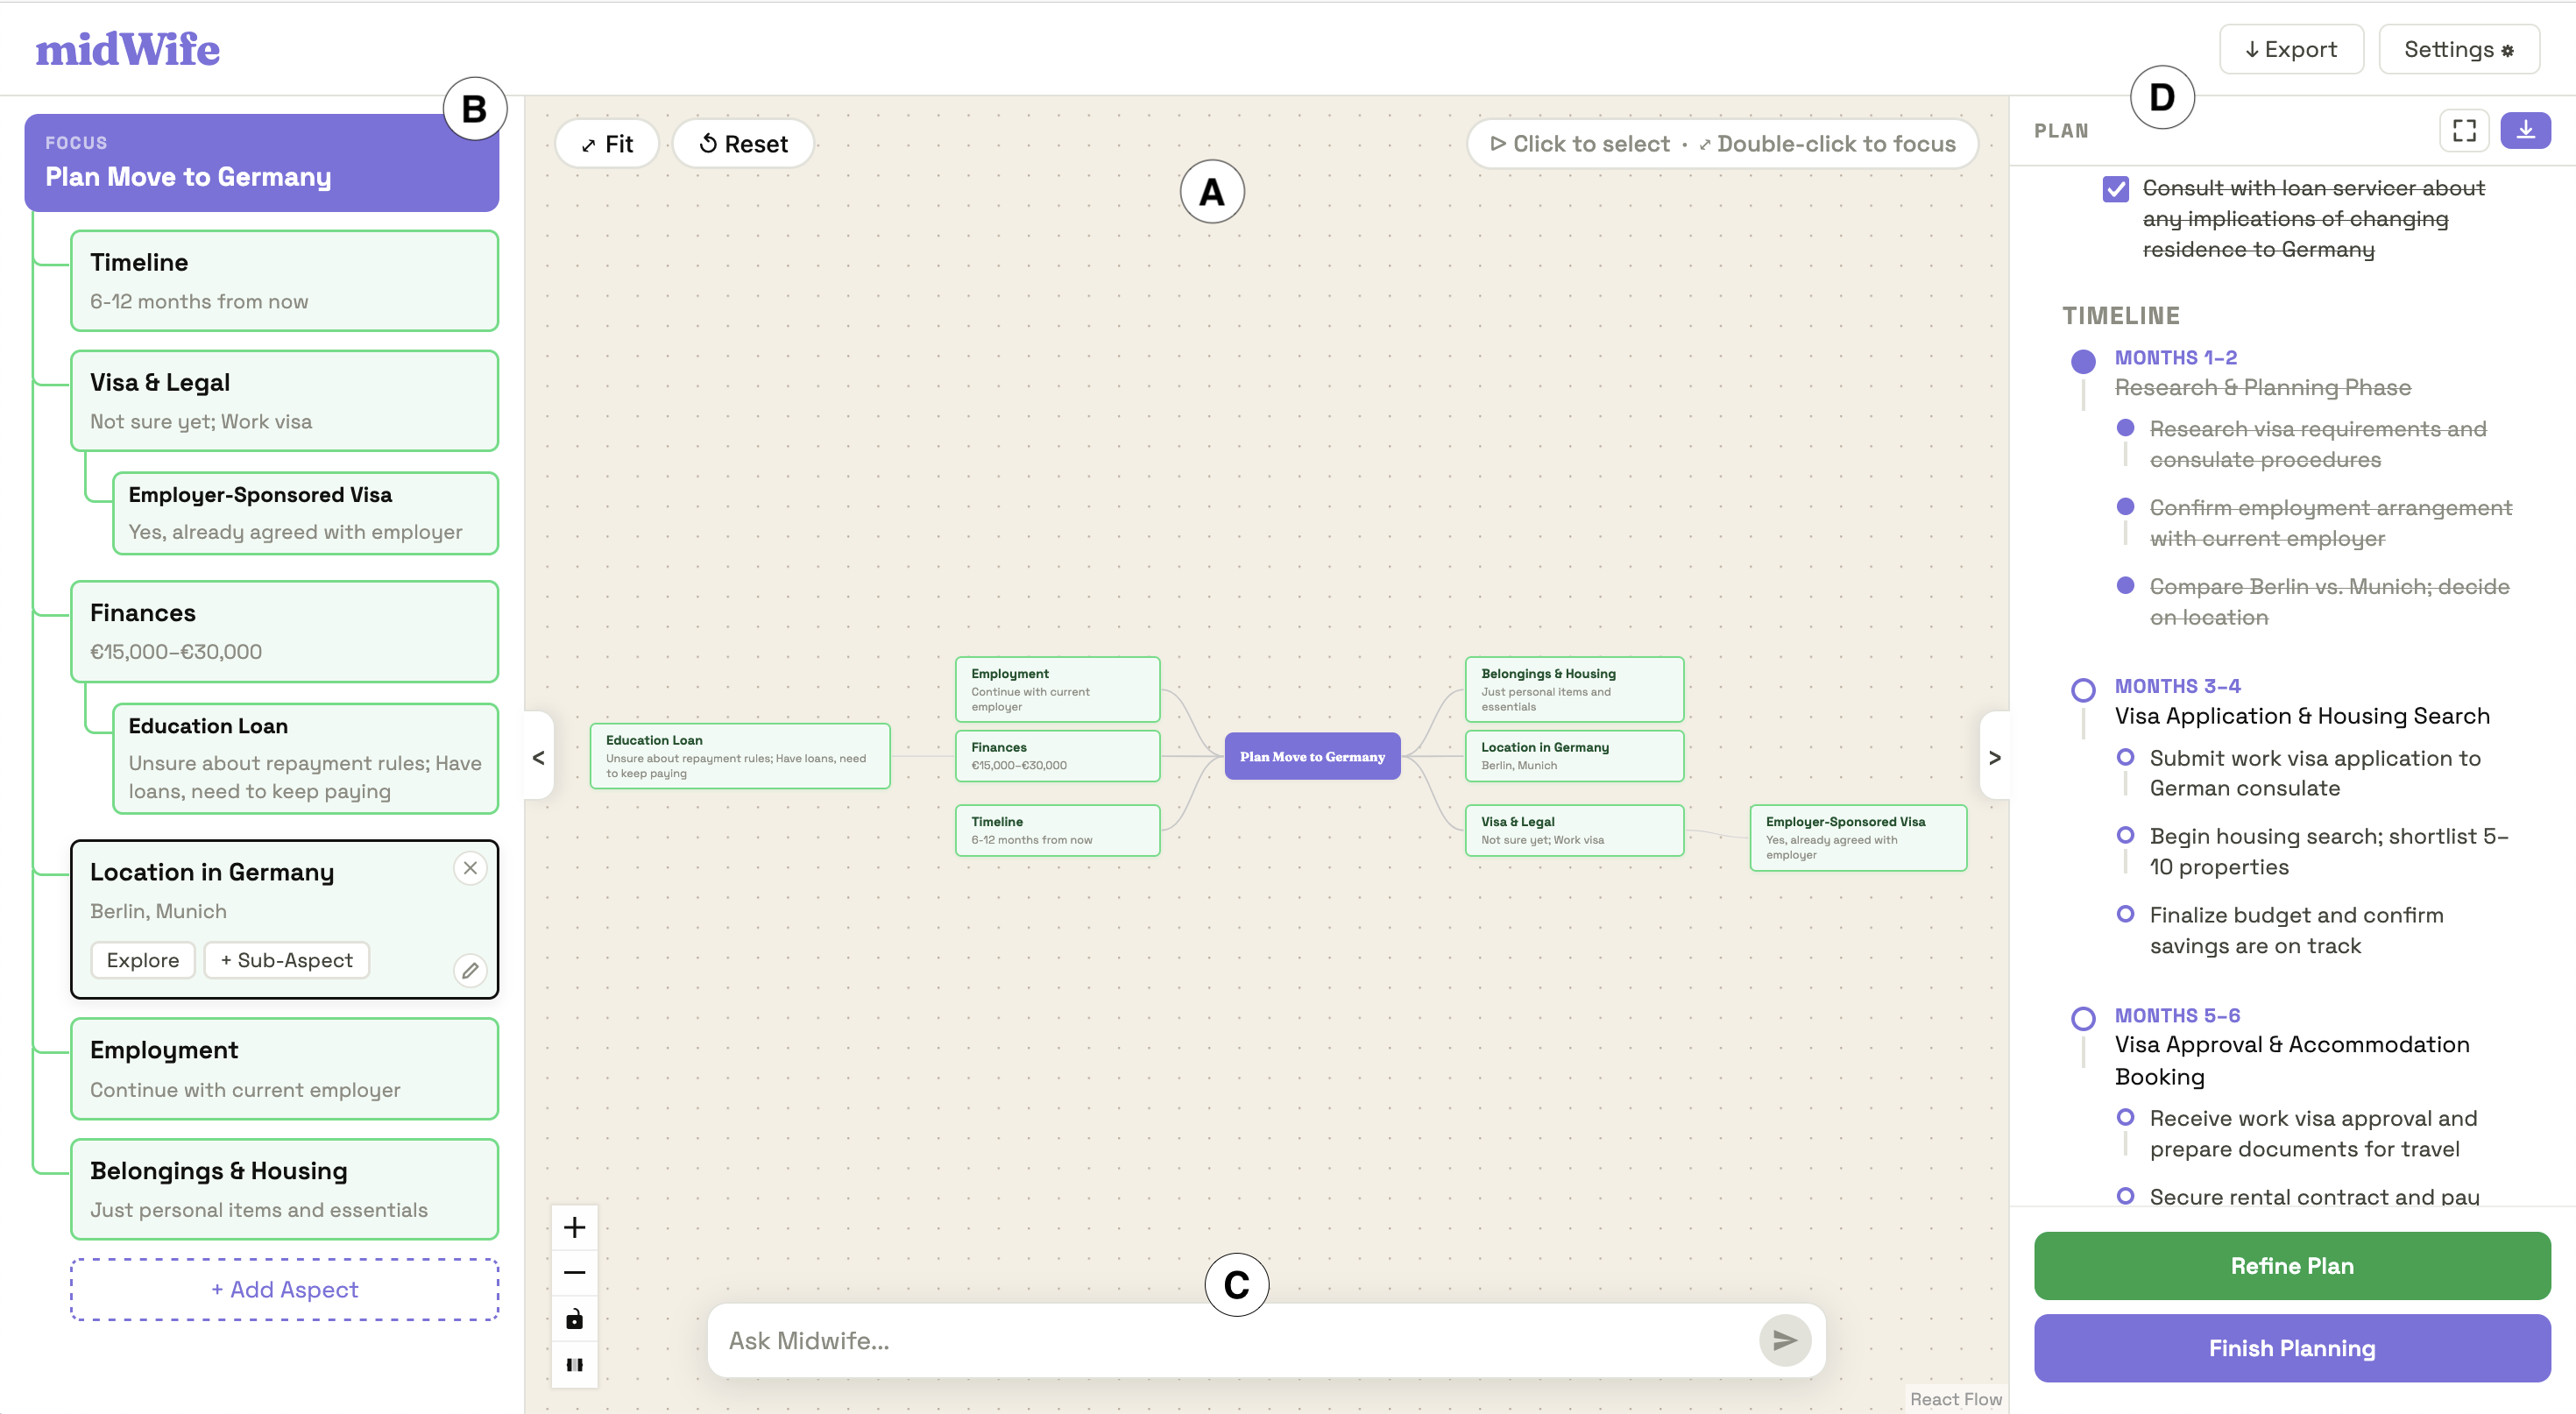
\includegraphics[width=\textwidth]{figures/teaser}
  \caption{The MidWife discourse canvas. A user's planning objective is decomposed
  into AI-generated Aspects — focused Socratic questions across key dimensions.
  Users answer via suggestion chips or free text; the tree expands recursively on
  elaboration. A per-node chat assistant (centre) guides the user to a concrete
  answer. The synthesis panel (right) distils the full discourse into actionable
  summaries adapted to the selected planning mode.}
  \Description{Screenshot of the MidWife interface showing a radial tree of
  planning Aspect nodes on a dark canvas, a chat panel anchored to the selected
  node, and a structured synthesis panel on the right side.}
  \label{fig:teaser}
\end{teaserfigure}

\maketitle

%% ═══════════════════════════════════════════════════════════════════════════════
\section{Introduction}
%% ═══════════════════════════════════════════════════════════════════════════════
%%
%% TARGET: ~400 words / ~0.65 column.
%%
%% Paragraph 1 — The problem (2–3 sentences)
%%   LLMs are increasingly used for complex, multi-dimensional thinking tasks —
%%   planning an event, making a career decision, working through a design problem.
%%   Yet every major LLM interface is a flat, scrollable chat thread: a single
%%   linear sequence that cannot represent the branching structure of real
%%   deliberation. Breadth is sacrificed for conversational flow.
%%
%% Paragraph 2 — The insight (2–3 sentences)
%%   The Socratic Method externalises thinking via structured questioning that
%%   surfaces hidden assumptions and maps the space of a problem before committing
%%   to answers [Kunz 1970, Toulmin 1958, Rittel 1973]. Applied to HCI, this
%%   lineage produced argument mapping tools (IBIS, Compendium) and, more recently,
%%   AI-powered dialectical systems [Tanprasert 2024, Chiang 2024]. These remain
%%   either structurally flat or AI-passive. What is missing is a system that
%%   combines spatial discourse structure with AI-as-Socratic-interlocutor.
%%
%% Paragraph 3 — What MidWife does (3–4 sentences)
%%   MidWife is a web application where users state a planning objective and select
%%   a planning mode. An LLM generates a set of Aspects — targeted Socratic
%%   questions — which form the root of a discourse tree. Users answer each
%%   Aspect; answering triggers elaboration into child Aspects. A per-node chat
%%   assistant guides the user toward a concrete answer. After exploring the tree,
%%   a synthesis panel distils the discourse into structured, actionable output.
%%
%% Paragraph 4 — Contributions (use \begin{itemize})
%%   \item The MidWife system: a working prototype of LLM-powered Socratic
%%         planning via interactive discourse trees.
%%   \item A mode-aware questioning engine supporting 9 distinct planning contexts,
%%         each modulating the AI's questioning strategy.
%%   \item A mixed-initiative interaction model in which user and AI jointly
%%         construct and refine the discourse tree.
%%   \item Design insights from building and iterating on the prototype, including
%%         a proposed evaluation plan for future work.
%%
Planning complex, multi-dimensional tasks is an increasingly common yet poorly
supported use case for large language models. Whether deciding how to change careers,
organizing a major event, or working through a research hypothesis, users routinely
turn to LLM-powered chat assistants as thinking partners~\cite{collins2024thoughtpartners}.
Yet every major LLM interface organizes interaction as a flat, scrollable chat thread
--- a one-dimensional medium that cannot represent the branching, recursive structure
of real deliberation~\cite{lee2025criticalthinking}. A user who spends hours in a
chat session planning a complex project has no spatial overview of what has been
considered, no ability to navigate across parallel concerns, and no persistent artifact
to return to and refine. Doing so with text-heavy media quickly becomes clunky; further,
a user who wishes to explore a tangent cannot do so without polluting the shared context
and potentially derailing the main thread of discussion. The \textit{scope} of the
discourse outgrows what the \textit{interface} can hold.

The Socratic Method has long provided an answer to this kind of open-ended inquiry.
Rather than providing answers, a skilled interlocutor asks focused questions that
surface hidden assumptions, expose logical gaps, and map the conceptual space of a
problem before any commitment is made~\cite{toulmin1958argument, schon1983reflective}.
Socrates himself described this role as that of an ``intellectual midwife'': whereas
midwives help give birth to children, his questioning helped give birth to wisdom and
ideas in others~\cite{plato_theaetetus}. Applied to interactive systems, this lineage
produced argument mapping tools rooted in Rittel and Kunz's
IBIS~\cite{kunz1970ibis, rittel1973wicked}, and more recently AI-powered dialectical
systems~\cite{tanprasert2024debate, chiang2024devilsadvocate}. What remains missing
is a single system that combines \textit{spatial discourse structure} with
\textit{AI-as-Socratic-interlocutor} --- one where questioning drives the growth of
a persistent, navigable tree of thinking.

We present \textbf{midWife}\footnote{The name is a direct tribute to the Socratic
metaphor: an AI interlocutor that helps users bring their plans and ideas into being,
much as Socrates helped his interlocutors give birth to wisdom.}: an interactive
web application for open-ended planning via Socratic dialogue. Users state a planning
objective and optionally select a \textit{mode} (logistics, brainstorming, creative,
decision, research, and more). midWife responds with a set of \textit{Aspects} ---
targeted Socratic questions spanning key dimensions of the objective --- rendered as
nodes in a branching discourse tree. Answering an Aspect (via suggestion chips or
free text) unlocks \textit{Elaboration}, which generates child Aspects conditioned
on the parent's answer and full ancestry context. A per-node chat assistant guides
users through difficult questions, surfacing new Aspects or reframing questions as
needed. As the tree grows, a \textit{Synthesis Panel} distils the full discourse into
structured, actionable output --- timelines, task lists, open questions --- adapted
to the selected planning mode. The entire tree is a persistent, resumable artifact.

This paper makes the following contributions:
\begin{itemize}
  \item \textbf{midWife}: a working prototype of LLM-powered Socratic planning
        via interactive discourse trees, built with a React + ReactFlow frontend
        and a FastAPI backend.
  \item A \textbf{mode-aware questioning engine} supporting nine distinct planning
        contexts, each modulating the AI's Socratic questioning strategy.
  \item A \textbf{mixed-initiative interaction model} in which user and AI jointly
        construct, navigate, and refine the discourse tree~\cite{horvitz1999mixedinitiative}.
  \item \textbf{Design insights} from iterative prototype development, including a
        proposed evaluation plan for future work.
\end{itemize}


%% ═══════════════════════════════════════════════════════════════════════════════
\section{Related Work}
%% ═══════════════════════════════════════════════════════════════════════════════
%%
%% TARGET: ~1.4 columns total.
%%
%% Each subsection should: summarise the thread in 3–4 sentences, cite 3–5
%% key papers, and end with one sentence pointing to the gap MidWife addresses.

%% ── 2.1 ───────────────────────────────────────────────────────────────────────
\subsection{AI-Augmented Sensemaking and Planning Tools}
%%
%% Papers to cite (in rough order of relevance):
%%   \cite{suh2023sensecape}      — hierarchical spatial LLM sensemaking (UIST 2023)
%%   \cite{ma2025deliberation}    — Human-AI Deliberation (CHI 2025) — closest conceptually
%%   \cite{liu2024selenite}       — structured overview + cold-start sensemaking (CHI 2024)
%%   \cite{suh2024luminate}       — design-space exploration with LLMs (CHI 2024)
%%   \cite{jiang2023graphologue}  — LLM responses as interactive diagrams (UIST 2023)
%%   \cite{kang2023synergi}       — mixed-initiative scholarly synthesis (UIST 2023)
%%
%% Throughline: these tools help users organise information spatially or
%% hierarchically, but AI produces *content* rather than *questions*. None
%% acts as a Socratic interlocutor that challenges the user's reasoning.
%% MidWife adds dialectical questioning to the spatial sensemaking paradigm.
%%
A wave of systems published at UIST and CHI since 2022 have directly addressed the
limitation of linear chatbot interfaces for complex information work. Sensecape~\cite{suh2023sensecape}
provides an infinite canvas where users interact with an LLM through multilevel
abstraction, moving fluidly between information foraging and sensemaking loops; a
within-subjects study found users explored significantly more topics and structured
knowledge more effectively than with a ChatGPT-plus-canvas baseline. Selenite~\cite{liu2024selenite}
solves the ``cold-start'' problem in unfamiliar decision domains by generating
structured overviews of options and criteria upfront, dynamically contextualizing
new information within those structures and accelerating information processing by
36\% across three studies. Luminate~\cite{suh2024luminate} prevents premature
convergence by first extracting key dimensions from a prompt, then generating
responses that span the resulting design space; a study with 14 professional writers
showed substantially increased divergent thinking. Graphologue~\cite{jiang2023graphologue}
converts LLM responses into interactive node-link diagrams in real time, demonstrating
that graphical, non-linear dialogue improves information parsing and exploration.
Synergi~\cite{kang2023synergi} exemplifies mixed-initiative scholarly sensemaking:
user-highlighted text seeds AI-generated hierarchical research threads grounded in
citation context. Most closely aligned is the Human-AI Deliberation system of Ma et
al.~\cite{ma2025deliberation}, which engages users in dimension-level opinion exchange
and iterative discussion rather than presenting static recommendations --- outperforming
traditional explainable AI in fostering appropriate reliance.

Beyond the academic literature, a growing class of commercial mind-mapping and planning
tools has begun integrating LLMs in this space. Tools such as Whimsical AI, Miro AI,
and various Notion-based workflows typically offer one of two interaction patterns:
(i)~the user provides a short prompt or intent and the tool generates a complete mind-map
or document in a single shot; or (ii)~the user uploads an existing artefact --- a PDF,
transcript, or note --- and the tool extracts a structured map from it. Neither pattern
is interactive in the deliberative sense. In the first, the AI does all the thinking and
the user is a passive recipient; in the second, the AI merely reorganises existing
material. In both cases, the user's agency is limited to accepting, rejecting, or lightly
editing the AI's output. The co-creative, back-and-forth quality of genuine planning ---
the iterative questioning, the gradual crystallization of vague intent into concrete
decisions --- is absent. As a consequence, users report lower sense of ownership over
the produced artefact. midWife's design is explicitly a response to this pattern: its
core invariant is that \textit{the AI never makes decisions on the user's behalf}.

A common thread across both academic systems and commercial tools is that AI produces
\textit{content}: information, structure, synthesis. It organises and generates; it does
not interrogate. midWife's core departure is that its primary AI role is to
\textit{ask}, not to tell.

%% ── 2.2 ───────────────────────────────────────────────────────────────────────
\subsection{Socratic and Dialectical AI Interaction}
%%
%% Papers to cite:
%%   \cite{tanprasert2024debate}    — debate chatbots + critical thinking (CHI 2024 Best Paper)
%%   \cite{chiang2024devilsadvocate}— interactive devil's advocate (IUI 2024)
%%   \cite{lim2026iffyornot}        — Socratic questioning + fallacy detection (TOCHI 2026)
%%   \cite{liu2024socraticlm}       — SocraticLM fine-tuned for Socratic teaching (NeurIPS 2024)
%%   \cite{lee2025criticalthinking} — GenAI reduces critical thinking (CHI 2025)
%%   \cite{collins2024thoughtpartners}— AI as thought partners (Nature 2024)
%%
%% Throughline: these systems question and challenge users effectively, but
%% operate within flat, linear chat interfaces. There is no persistent spatial
%% representation of the evolving discourse. MidWife embeds Socratic interaction
%% inside a structured discourse tree.
%%
Tanprasert et al.~\cite{tanprasert2024debate} demonstrated in a landmark CHI 2024 Best
Paper that LLM-powered debate chatbots with outgroup identity and persuasive rhetoric
most effectively induced critical thinking --- interpretation, analysis, and
self-regulation --- in users engaging with online video content. Chiang et
al.~\cite{chiang2024devilsadvocate} showed that interactive devil's advocate agents
that challenge AI recommendations improved appropriate reliance and decision accuracy
by catalyzing extended discussion. Lim et al.~\cite{lim2026iffyornot} combined fallacy
detection with Socratic questioning in a browser extension, reporting that it encourages
attentiveness and poses thought-provoking questions in evaluation of potential
misinformation. At the model level, SocraticLM~\cite{liu2024socraticlm} fine-tunes
LLMs for Socratic teaching through a multi-agent pipeline, producing a dataset of 35K
Socratic dialogues --- validating that LLMs can reliably ask guiding questions rather
than give answers at scale. Chang~\cite{chang2023socratic} engineers ten Socratic
strategies from Plato's dialogues (elenchus, maieutics, dialectic, counterfactual
reasoning) into prompt templates, demonstrating improved output correctness and more
critically examined responses. Lee et al.~\cite{lee2025criticalthinking} provide an
empirical motivation for midWife's design: surveying 319 knowledge workers, they find
higher AI confidence correlates with \textit{less} critical engagement by users ---
underscoring the need for AI systems that provoke thought rather than satisfy it.
Collins et al.~\cite{collins2024thoughtpartners} frame the aspirational target as AI
``thought partners'': reasonable, insightful, trustworthy collaborators that think
\textit{with} humans.

A shared limitation across this stream is structural: these systems operate within
flat, linear chat interfaces. The dialogue may be dialectical, but the representation
is one-dimensional. midWife embeds Socratic questioning inside a persistent, spatial
discourse tree --- giving the dialogue a structure that users can navigate, revisit,
and build upon.

%% ── 2.3 ───────────────────────────────────────────────────────────────────────
\subsection{Non-Linear Conversation and Argumentation}
%%
%% Papers to cite:
%%   \cite{kunz1970ibis}          — IBIS: issues/positions/arguments (1970)
%%   \cite{conklin1988gibis}      — gIBIS: first graphical IBIS tool (1988)
%%   \cite{rittel1973wicked}      — wicked problems require deliberative process
%%   \cite{toulmin1958argument}   — Toulmin argument model
%%   \cite{zhang2023visar}        — VISAR: visual argument tree + LLM sparks (UIST 2023)
%%   \cite{pan2025amquestioner}   — AMQuestioner: argument maps + Socratic chat (CSCW 2025)
%%   \cite{wang2025nodetree}      — node-tree beats chatbot for decision/brainstorm tasks
%%   \cite{horvitz1999mixedinitiative} — principles of mixed-initiative UI (CHI 1999)
%%
%% Throughline: this lineage provides structured argument representations but
%% historically lacked AI facilitation. Recent work (VISAR, AMQuestioner) begins
%% integrating LLMs for content generation, but not as Socratic facilitators.
%% MidWife synthesises all three threads.
%%
The intellectual lineage of structured discourse tools begins with Kunz and Rittel's
IBIS~\cite{kunz1970ibis}, which defined a grammar for structuring complex policy
deliberation around Issues (questions), Positions (answers), and Arguments (pros/cons).
Rittel and Webber's complementary ``wicked problems'' work~\cite{rittel1973wicked}
established why such structure is necessary: ill-structured problems demand argumentative,
deliberative processes rather than algorithmic resolution. Toulmin's argument
model~\cite{toulmin1958argument} contributed a richer grammar (claim, grounds, warrant,
backing, qualifier, rebuttal) that underpins virtually all subsequent computational
argumentation work. Conklin and Begeman's gIBIS~\cite{conklin1988gibis} realized IBIS
graphically, demonstrating that typed structure eliminates unconstructive conversational
moves; Compendium extended this into a professional dialogue-mapping practice.
MacLean et al.'s QOC notation~\cite{maclean1991qoc} showed a structurally isomorphic
pattern (Questions, Options, Criteria) for design rationale, confirming the generality
of branching deliberation structures. Cognitive grounding comes from Russell et al.'s
sensemaking cost model~\cite{russell1993sensemaking} and Pirolli and Card's dual-loop
foraging-sensemaking framework~\cite{pirolli2005sensemaking}: explicit tree representations
reduce the cognitive cost of organizing complex thought by externalising working memory.

Recent work has begun augmenting this lineage with LLMs. VISAR~\cite{zhang2023visar}
supports argumentative writing through hierarchical goal brainstorming and LLM-powered
``argumentation sparks'' (counterarguments, evidence, logical weakness detection) within
a tree-structured outline. AMQuestioner~\cite{pan2025amquestioner} automatically extracts
argument maps from online discussions and presents Socratic questions to guide users in
critically exploring claims; a study of 24 participants showed improved critical thinking
skills and open-mindedness. Wang et al.~\cite{wang2025nodetree} provide direct empirical
support for midWife's design choice: node-tree interfaces outperformed chatbots specifically
on \textit{decision-making} and \textit{brainstorming} tasks, with 90\% of node-tree users
finding the interface easy to navigate. Horvitz's mixed-initiative
principles~\cite{horvitz1999mixedinitiative} supply the interaction design framework for
managing when the AI should take initiative versus deferring to the user.

Despite this progress, these systems use AI primarily for \textit{content generation}:
surfacing counterarguments, labelling argument types, retrieving evidence. None positions
the AI as a \textit{Socratic facilitator} whose primary goal is to help the user think
more deeply through structured questioning.

%% ── 2.4 Positioning ───────────────────────────────────────────────────────────
%%
%% Write 3–4 sentences (or a small table) making the gap explicit:
%% Three streams are active, but no current system integrates:
%%   (1) Spatial/hierarchical discourse structure
%%   (2) AI as Socratic interlocutor (questioner, not answer machine)
%%   (3) Mode-aware questioning across diverse planning contexts
%% Consider a 3-column comparison table:
%%   System | Spatial structure | Socratic AI | Mode-aware
%% Then one sentence: "MidWife's contribution is the synthesis of these three."
%%
The three threads described above are active and productive, yet no existing system
integrates all three. Table~\ref{tab:positioning} characterizes the landscape.
Sensemaking tools provide spatial or hierarchical structure but the AI generates
\textit{content}, not questions. Dialectical AI systems challenge and interrogate but
do so within flat, linear interfaces. Argumentation tools provide structured discourse
representations but use AI only for content generation, not Socratic facilitation.
midWife's contribution is the synthesis: a tree-structured dialogue interface where
the AI acts as a Socratic interlocutor, combining the spatial structure of Sensecape
and Graphologue, the dialectical AI role of Human-AI Deliberation and the debate
chatbot literature, and the argument grammar of IBIS and Toulmin --- extended with
mode-aware questioning across nine distinct planning contexts.

\begin{table}[h]
\caption{Positioning of midWife relative to representative prior systems.
\checkmark~= fully present, $\sim$~= partial, $\times$~= absent.}
\label{tab:positioning}
\small
\begin{tabular}{p{3.2cm}ccc}
\toprule
\textbf{System} & \textbf{Spatial tree} & \textbf{Socratic AI} & \textbf{Mode-aware} \\
\midrule
Sensecape \cite{suh2023sensecape}               & \checkmark & $\times$   & $\times$ \\
Human-AI Deliberation \cite{ma2025deliberation} & $\times$   & $\sim$     & $\times$ \\
Debate Chatbots \cite{tanprasert2024debate}      & $\times$   & \checkmark & $\times$ \\
VISAR \cite{zhang2023visar}                      & \checkmark & $\sim$     & $\times$ \\
AMQuestioner \cite{pan2025amquestioner}          & \checkmark & $\sim$     & $\times$ \\
\midrule
\textbf{midWife (ours)}                          & \checkmark & \checkmark & \checkmark \\
\bottomrule
\end{tabular}
\end{table}


%% ═══════════════════════════════════════════════════════════════════════════════
\section{MIDWIFE}
%% ═══════════════════════════════════════════════════════════════════════════════
%%
%% TARGET: ~1.5 columns.

%% ── 3.1 ───────────────────────────────────────────────────────────────────────
\subsection{Motivating Scenario}

Consider Priya, a software engineer contemplating a move abroad for a new career
opportunity. She opens a chat assistant and types her situation --- and immediately
faces the core problem: a good answer requires exploring dozens of interconnected
dimensions. What is her financial runway? Does she have the right visa? What happens
to her current apartment and social network? What are her priorities --- career growth,
lifestyle, proximity to family? A linear chat thread surfaces some of these concerns,
but has no way to hold them simultaneously. Exploring one thread buries earlier ones.
A good follow-up about housing arrives twenty messages after the topic was first raised;
the context is effectively stale. Worse, when Priya wants to take a quick tangent ---
say, a digression about her lease terms --- she cannot do so without polluting the
shared context and derailing the main thread.

With midWife, Priya types: ``I'm thinking of moving to Berlin for a job opportunity''
and selects the \textit{Decision} mode. midWife generates five Aspects: \textit{Finances},
\textit{Visa \& Logistics}, \textit{Career Fit}, \textit{Lifestyle}, and
\textit{Family \& Social}. Each appears as a node on a radial discourse canvas. She
clicks \textit{Finances}: midWife asks, ``How long could you sustain yourself financially
if you spent a few months settling in before starting?'' She types her answer. She clicks
\textit{Elaborate} --- midWife generates three child Aspects: \textit{Cost of Living},
\textit{Savings Buffer}, and \textit{Currency Risk}. She navigates back up and clicks
\textit{Career Fit}, opening the per-node chat assistant. She is unsure how to think
about this angle; the assistant asks, ``What would you want to have achieved professionally
in two years that your current role does not allow?'' --- guiding her to a concrete answer
without providing one. After exploring four of the five top-level Aspects, she clicks
\textit{Synthesise}. midWife produces a structured Decision Panel: an overview, a list
of open questions, a recommendation summary, and actionable next steps. Priya did not
\textit{receive} a plan --- she \textit{built} one.

%% ── 3.2 ───────────────────────────────────────────────────────────────────────
\subsection{Design Goals}
%%
%% Derive each goal directly from the literature gaps in Section 2.
%% Suggested goals (3–5 sentences, one per goal):
%%
%%   DG1 — Represent deliberation spatially:
%%     Model complex planning as a traversable, branching discourse tree so
%%     users can see and navigate the full problem space at once.
%%     (Motivated by: Sensecape, Graphologue, node-tree study.)
%%
%%   DG2 — AI as Socratic facilitator, not oracle:
%%     The AI's role is to ask focused, well-formed questions — not to supply
%%     answers. Users should arrive at their own conclusions through structured
%%     reflection. (Motivated by: Human-AI Deliberation, SocraticLM, Wood 1976.)
%%
%%   DG3 — Support diverse planning contexts:
%%     The meaning of a "good clarifying question" depends radically on context.
%%     The system must modulate its questioning strategy per planning mode.
%%     (Motivated by: Shaping Scaffolding [Bhat 2024], mode diversity observed
%%     in early prototype testing.)
%%
%%   DG4 — Mixed-initiative tree construction:
%%     Both user and AI should be able to add, remove, move, and relabel nodes.
%%     (Motivated by: Horvitz 1999 mixed-initiative principles.)
%%
%%   DG5 — Discourse as persistent, resumable artifact:
%%     The tree is not a transient chat log but a document that users can return
%%     to, continue, and eventually synthesise. (Motivated by: Fuse [Kuznetsov
%%     2022], Distributed Cognition [Hutchins 1995].)
%%
\textbf{D1 --- Visualize Discourse as a Dynamic Map of Thinking.}
A linear chat transcript cannot externalize the structure of multi-dimensional thinking.
Our first goal was to find a better \textit{medium}: one in which the growing discourse
is visible as a spatial artefact the user can navigate. Given the user's planning
objective, midWife polls the LLM for the five or six most pertinent \textit{Aspects}
worth exploring. Each becomes a node in a radial graph, with the user's Thesis (their
original intent or objective) at the centre and Aspects as immediate children. As the
user answers questions and elaborates branches, the tree grows outward, accumulating
a visual record of what has been considered, decided, and left open. A Navigator Pane
on the left of the interface allows users to add, edit, move, and delete nodes at any
time, ensuring the map remains theirs to shape.

\textbf{D2 --- Probe, Rather Than Answer, on the User's Behalf.}
Many contemporary mind-mapping and planning tools offload the thinking away from the
user entirely: the user provides an initial intent and is presented with a complete
plan, map, or document generated by the AI. While efficient, this pattern significantly
diminishes the user's \textit{sense of ownership} over the produced artefact --- the
final outcome does not carry their fingerprint. We take a fundamentally different
approach. midWife uses the LLM exclusively to: (i)~ask probing questions; (ii)~uncover
hidden assumptions; (iii)~help the user verbalize inchoate ideas through focused
follow-ups; and (iv)~offer concrete suggestions only when the user is navigating an
unfamiliar domain. The \textit{onus} of deciding, committing, and directing always
rests with the user. This design choice is testable: we expect users to report higher
agency, ownership, and satisfaction with the output than users of single-shot generation
tools --- a hypothesis for future evaluation.

\textbf{D3 --- Model Thinking as a Mixed-Initiative Dialogue.}
Effective deliberation is neither fully user-driven nor fully AI-driven; it is a
back-and-forth in which each party contributes what the other cannot easily do alone.
We therefore designed midWife so that \textit{every significant action} can be initiated
by either the user or the AI. New Aspects can be AI-generated (via elaboration) or
user-created (via the Navigator Pane or manual node creation). Questions can be
AI-authored or user-edited. The Synthesis Panel is initially generated by the AI based
on the completed discourse, but the user retains full executive control: they can edit,
delete, or redirect any section of the plan via natural language chat. This mirrors
the core principles articulated by Horvitz~\cite{horvitz1999mixedinitiative}: the
system should scope its initiative to the user's current context, offer safety nets
(e.g. editable suggestions), and time AI interventions to moments when the user is
most likely to benefit from them.

%% ── 3.3 ───────────────────────────────────────────────────────────────────────
\subsection{The Discourse Tree Model}
%%
%% Describe the data model concisely (this is architecture, not implementation).
%%
%%   Root node: the user's planning objective (the "thesis").
%%   Aspect nodes: each has an aspect label (≤3 words), a Socratic question,
%%     3–5 pre-generated answer suggestions, and an optional free-text answer.
%%   Children: generated on elaboration, scoped to the parent's domain.
%%   Tree construction: answering an Aspect unlocks elaboration; elaboration
%%     generates child Aspects whose questions are conditioned on the full
%%     ancestry path (context_path injection).
%%
%%   Two special node states worth explaining:
%%     Ghost nodes: children pre-fetched in the background after an answer is
%%       submitted, hidden until the user elaborates. Reduces perceived latency.
%%     Recontextualization: as a branch grows, ancestor labels may become
%%       misleading relative to their children's actual content. The system
%%       periodically checks and proposes updated labels.
%%
%%   Connect to theory:
%%     AspectNode maps to IBIS Issues [Kunz 1970] and Toulmin's claim/grounds
%%     [Toulmin 1958]. The context_path injection mirrors the sensemaking loop's
%%     representation-refinement cycle [Russell 1993, Pirolli 2005].
%%

Each session in midWife is called a \textbf{\textit{Discourse}} --- a structured
planning session centred around a \textbf{\textit{Thesis}}: the user's objective,
intent, topic of interest, or open question. Before the Discourse begins, the user
specifies a \textbf{\textit{Mode of Help}}: one or more of Logistics, Brainstorm,
Creative, Problem-Solving, Decision, Research, Reflect, Set Goals, or Learn, which
shapes the AI's questioning strategy throughout.

The fundamental unit of the Discourse is an \textbf{\textit{Aspect}}: a dimension of
the Thesis that warrants exploration. Each Aspect is a node in the tree carrying four
fields: (i)~a short \textit{label} (at most three words, e.g.\ \textit{Budget},
\textit{Career Fit}); (ii)~a \textit{Socratic question} --- a focused,
beginner-friendly prompt to help the user think through that dimension; (iii)~a set
of three to five pre-generated \textit{suggestion chips}; and (iv)~the user's
\textit{answer}, once provided. Answering an Aspect unlocks \textit{Elaboration}:
midWife generates child Aspects whose questions are conditioned on the full
\textit{ancestry path} --- every aspect/question/answer triple from the root down to
the current node. This ensures deeper questions are meaningfully scoped to what the
user has already decided.

\textbf{Recontextualization} addresses a subtle issue that emerges as the discourse
deepens: an ancestor's short label may no longer accurately reflect the scope of its
subtree. The system periodically re-evaluates ancestor labels against their children's
content and proposes updated labels, keeping the map legible as the discourse grows.

%% ── 3.4 ───────────────────────────────────────────────────────────────────────
\subsection{User Interface \& Features}

After the user submits their Thesis and Mode of Help, the interface transitions to the
main Discourse page, which consists of three primary areas: (i)~the \textbf{Navigator
Pane} on the left, showing a structured list of all \textit{Aspects} in the current
Discourse, allowing users to add, edit, move, and delete nodes at any time; (ii)~the
\textbf{Discourse Canvas} at the centre, a node-link diagram rendering the Thesis and
its Aspect nodes radially, updated in real time as the Discourse grows; and (iii)~the
\textbf{Plan Pane} on the right, displaying a rich Markdown summary of action items,
timelines, and open questions synthesised from the current state of the Discourse.

\subsubsection{Interview \& Answering}

For each \textit{Aspect} in the Discourse, midWife engages the user in an
\textbf{\textit{Interview}}: a focused, one-at-a-time question session. The user is
presented with the Socratic question for the selected Aspect alongside up to five
pre-filled suggestion chips. They may select one or more chips, add detail in a
free-text box, or type a fully custom answer. If they are uncertain how to approach the
question, they may choose \textit{Chat about this}, which opens the \textbf{Chat
Interface} anchored to that specific node. Here, the LLM helps the user articulate
their requirements, resolve ambiguity, and arrive at either a pre-specified option or
a custom answer of their own. Critically, the chat assistant does not answer the
question \textit{for} the user: it asks, clarifies, and guides until the user reaches
their own conclusion.

\subsubsection{Mode-Aware Questioning Engine}

midWife supports nine planning modes --- Logistics, Brainstorm, Creative,
Problem-Solving, Decision, Research, Reflect, Set Goals, and Learn --- each of which
injects a distinct instruction paragraph into the LLM's system prompt, redefining what
constitutes a relevant Socratic question for that context. Users may select a single
mode or combine multiple for hybrid sessions.

\subsubsection{Navigator Pane}

The Navigator Pane provides a structured list view of the Discourse, organised around
the concept of a \textbf{Focus Node}. By default the root Thesis is the Focus Node, and
the Pane displays it alongside up to its grandchildren --- giving users a bounded,
readable slice of the tree at any one time. Users may double-click any Aspect to
re-focus: the Canvas recentres on that node and the Pane narrows to its local subtree,
allowing deep branches to be explored without the surrounding tree becoming a distraction.

Within the Navigator Pane, users can add new Aspect nodes to any existing node or to the
Thesis itself, edit labels, delete nodes, and move a node to become the child of a
different parent if they feel the structure better reflects their thinking. Nodes can also
be expanded by the AI: each Aspect card carries an \textbf{Explore} button that instructs
midWife to generate additional directions to investigate under that Aspect, surfacing
branches the user may not have considered.

\subsubsection{Plan Pane}

While the Discourse Canvas captures the \textit{structure} of a user's thinking, the
Plan Pane synthesises its \textit{implications}. It surfaces information that the canvas
does not directly represent: concrete action items and \textsc{todo}s derived from
answered Aspects, a timeline if the user's objective has a temporal dimension,
open questions that remain unresolved in the tree, and risks or considerations that are
still unaddressed. All of this is rendered as a rich Markdown document, updated on demand
as the Discourse grows.

Users steer the Plan through the chat interface at the bottom of the Discourse Canvas.
Each requested edit --- rephrasing a section, adding a new consideration, restructuring
the timeline --- is first shown as a \textbf{diff preview}; the user can accept the
proposed changes or dismiss them and keep the current Plan. This accept/reject flow
ensures the Plan remains under the user's control rather than being silently overwritten
by the AI.

%% ── 3.5 ───────────────────────────────────────────────────────────────────────
\subsection{Mixed-Initiative Interaction}
%%
%% Frame around Horvitz [1999] principles.
%%
%% AI-led actions (when the system takes initiative):
%%   - Generates initial Aspects on session creation
%%   - Pre-generates suggestion chips (answer options) per node
%%   - Prefetches ghost children after an answer is submitted
%%   - Proposes ancestor re-labels via recontextualization
%%   - Synthesises the full tree into a structured summary panel on demand
%%
%% User-led actions (user takes initiative):
%%   - Answers via suggestions or free text
%%   - Selects which branches to elaborate
%%   - Manually adds, moves, deletes, and relabels nodes
%%   - Opens per-node chat to work through a hard question conversationally
%%   - Edits the synthesis panel via natural language directives
%%
%% Per-node chat is a key design decision worth elaborating:
%%   The chat assistant is scoped to a single node's context (aspect + question
%%   + full ancestry path + existing answers). It guides the user toward ONE
%%   concrete answer. It can surface new Aspects if the user raises genuinely
%%   new concerns. It can reframe the question if it doesn't fit the user.
%%   This scoping prevents context bleed and keeps the conversation focused —
%%   a deliberate departure from global chatbots.
%%
midWife distributes initiative between user and AI across every layer of the
interaction. On the AI side: the system generates the initial set of Aspects on
session creation; pre-generates suggestion chips for each node; proposes ancestor relabelling via
recontextualization; and synthesises the full discourse into the Plan Pane on demand.
On the user side: the user answers via chips or free text; selects which branches to
elaborate; manually adds, moves, deletes, and relabels nodes via the Navigator Pane;
opens the per-node chat for any question they find difficult; and edits the Plan Pane
via natural language directives in the chat interface.

A key design decision is scoping the chat assistant to individual nodes rather than
providing a single global chatbot. Each chat session is initialised with the full
context of the selected node --- its label, Socratic question, and the complete
ancestry path of prior answers --- and is given one directive: help the user reach a
concrete answer to \textit{this} question. The assistant will reframe the question if
the user finds it irrelevant, surface a new Aspect if a genuinely new concern emerges,
and extract a suggested answer as soon as the conversation converges. Each node's
chat history is preserved independently, allowing users to track the reasoning behind
any answer and return to prior conversations without losing context. This scoping
prevents context bleed across unrelated branches and ensures the chat always serves
the discourse tree rather than replacing it.

%% ═══════════════════════════════════════════════════════════════════════════════
\section{Implementation}
%% ═══════════════════════════════════════════════════════════════════════════════
%%
%% TARGET: ~1 column + 2 figures.
%%
%% Focus: implementation decisions that directly shaped the UX — not infra/ops details.
%%
%% Stack (brief): React + Vite + ReactFlow + Dagre (frontend), FastAPI (backend).
%%   ReactFlow: gives us free pan/zoom/select on the canvas; Dagre handles
%%   automatic tree layout so nodes never overlap as the tree grows.
%%   Session state stored in browser localStorage → resumable sessions without login.
%%
%% AI model choice and its UX implications:
%%   Claude Haiku 4.5 primary: low latency keeps the interview feel responsive;
%%   structured JSON output means aspect labels, questions, and chips arrive in one
%%   round-trip with no post-processing delay visible to the user.
%%   Gemini fallback chain: keeps the system available under rate limits without
%%   the user seeing an error — graceful degradation rather than a broken state.
%%
%% Prompt engineering decisions with UX consequences:
%%   - covered_aspects deduplication: existing tree labels injected as "do not
%%     repeat" context → user never sees a duplicate or near-duplicate node appear.
%%   - context_path injection: full ancestry injected per elaboration call →
%%     questions grow progressively more specific as the tree deepens, which users
%%     perceive as the system "understanding" where they are in their thinking.
%%   - Mode-specific system prompts: each of the 9 modes swaps in a different
%%     questioning persona and output schema (e.g. Research mode produces
%%     hypothesis/evidence/gap Aspects; Reflect mode produces more introspective
%%     questions) — the same interaction model feels meaningfully different per context.

\begin{figure}[h]
  \centering
  %% Replace with an architecture diagram:
  %%   [React/Vite Frontend] <→> [FastAPI Backend] <→> [Claude Haiku]
  %%                                                ↘> [Gemini fallbacks]
  %% Show the key REST endpoints (POST /session, /elaborate, /chat, /generate-panel)
  %% and the localStorage sync arrow from frontend.
  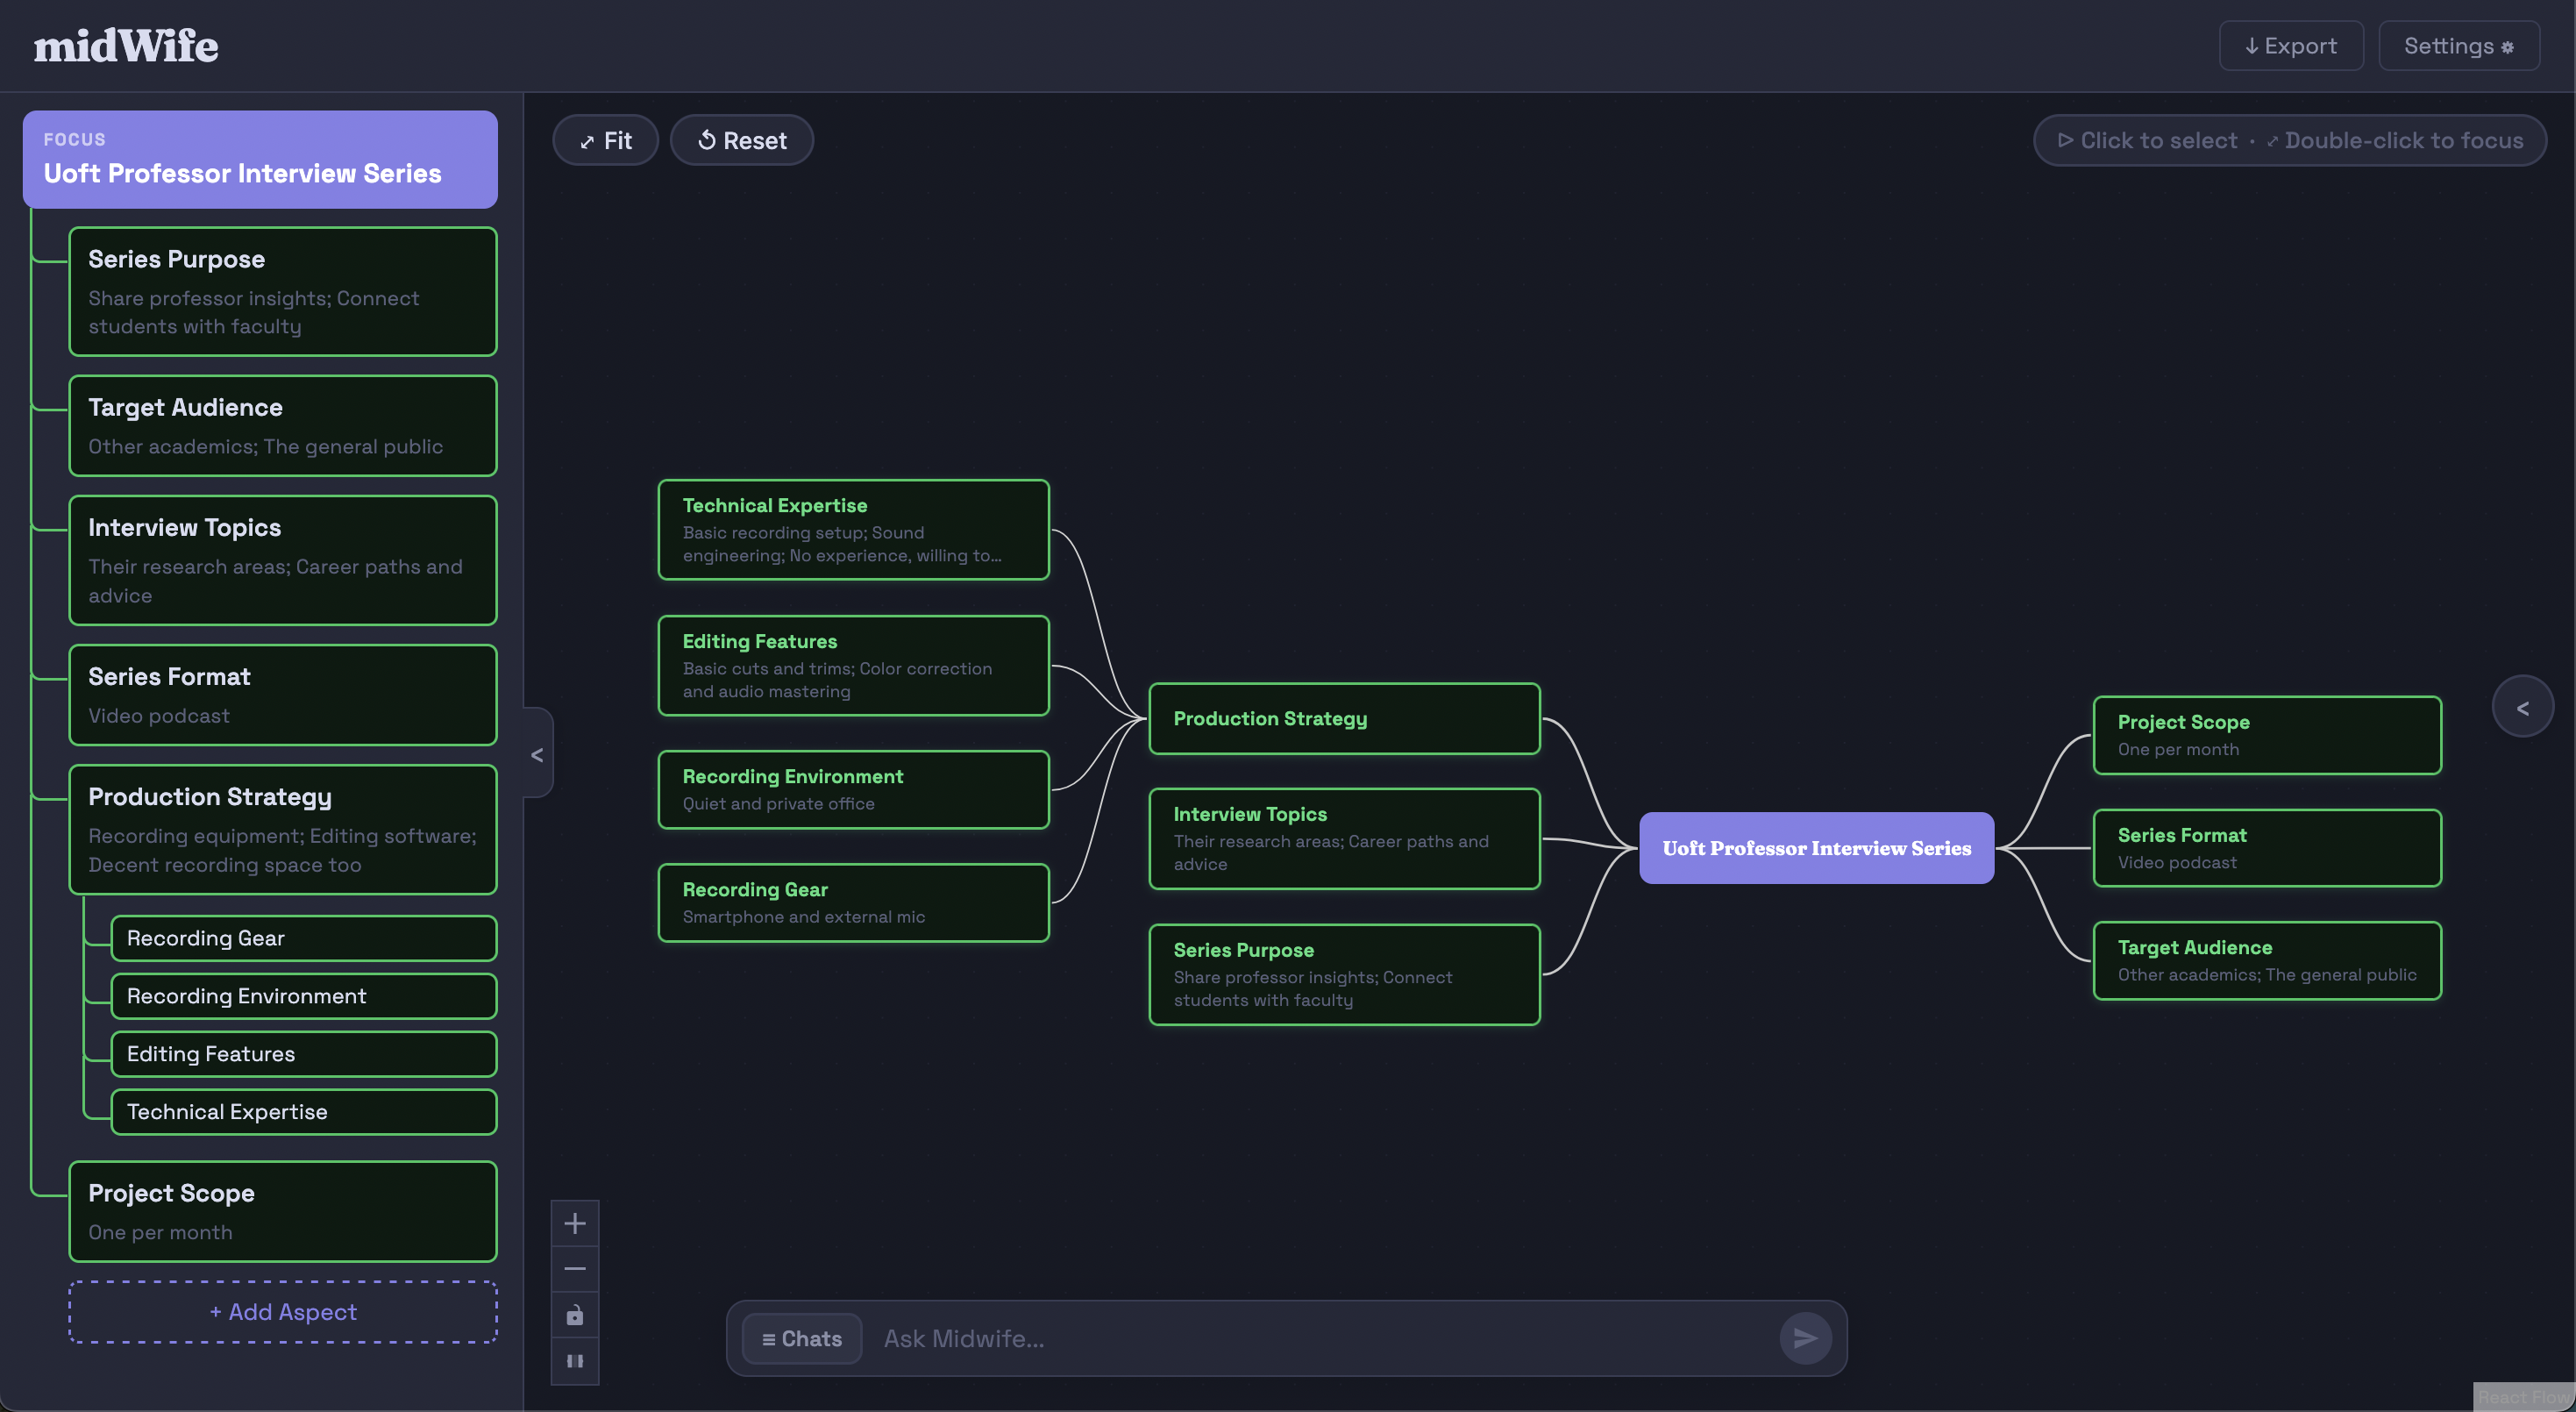
\includegraphics[width=\linewidth]{figures/architecture}
  \caption{MidWife system architecture. The React frontend communicates with a
  FastAPI backend over a REST API. Claude Haiku serves as the primary LLM;
  Gemini models provide a cascading fallback. Session state is maintained
  server-side and synced to browser localStorage, enabling resumable sessions
  without a database.}
  \Description{Architecture diagram showing React frontend connected via REST
  API to a FastAPI backend, which calls Claude Haiku with a fallback to three
  Gemini models. A bidirectional arrow between frontend and localStorage is shown.}
  \label{fig:architecture}
\end{figure}

%%
%% Usage scenario — walk through a concrete end-to-end example:
%%   1. User opens MidWife, enters objective (e.g. "Plan my sister's birthday"),
%%      selects "logistics" mode, optionally fills background fields.
%%   2. Backend generates 5–6 top-level Aspects (Budget, Venue, Guest List, …).
%%      Discourse canvas renders the tree; each node shows the Aspect label.
%%   3. User clicks a node → InterviewFlow opens: reads the Socratic question,
%%      sees 3–4 suggestion chips, selects one or types a free answer.
%%   4. Answering submits the answer; ghost children are prefetched silently.
%%      User clicks Elaborate → children are revealed as new Aspect nodes.
%%   5. For a difficult node, user opens chat → Midwife assistant asks follow-ups
%%      and eventually surfaces a suggested_answer the user can accept.
%%   6. After exploring key branches, user clicks Synthesise → the summary panel
%%      generates mode-specific tabs (Overview, Timeline, Tasks, Open Questions).
%%   7. User can chat with the panel to refine individual sections.
%%      Full session is resumable from the landing page via localStorage.
%%
%% Include Figure 2 here: a 2-panel composite screenshot — ideally showing
%% (a) a session mid-progress with several answered nodes,
%% (b) the synthesis panel with populated tabs.
%%
\begin{figure}[h]
  \centering
  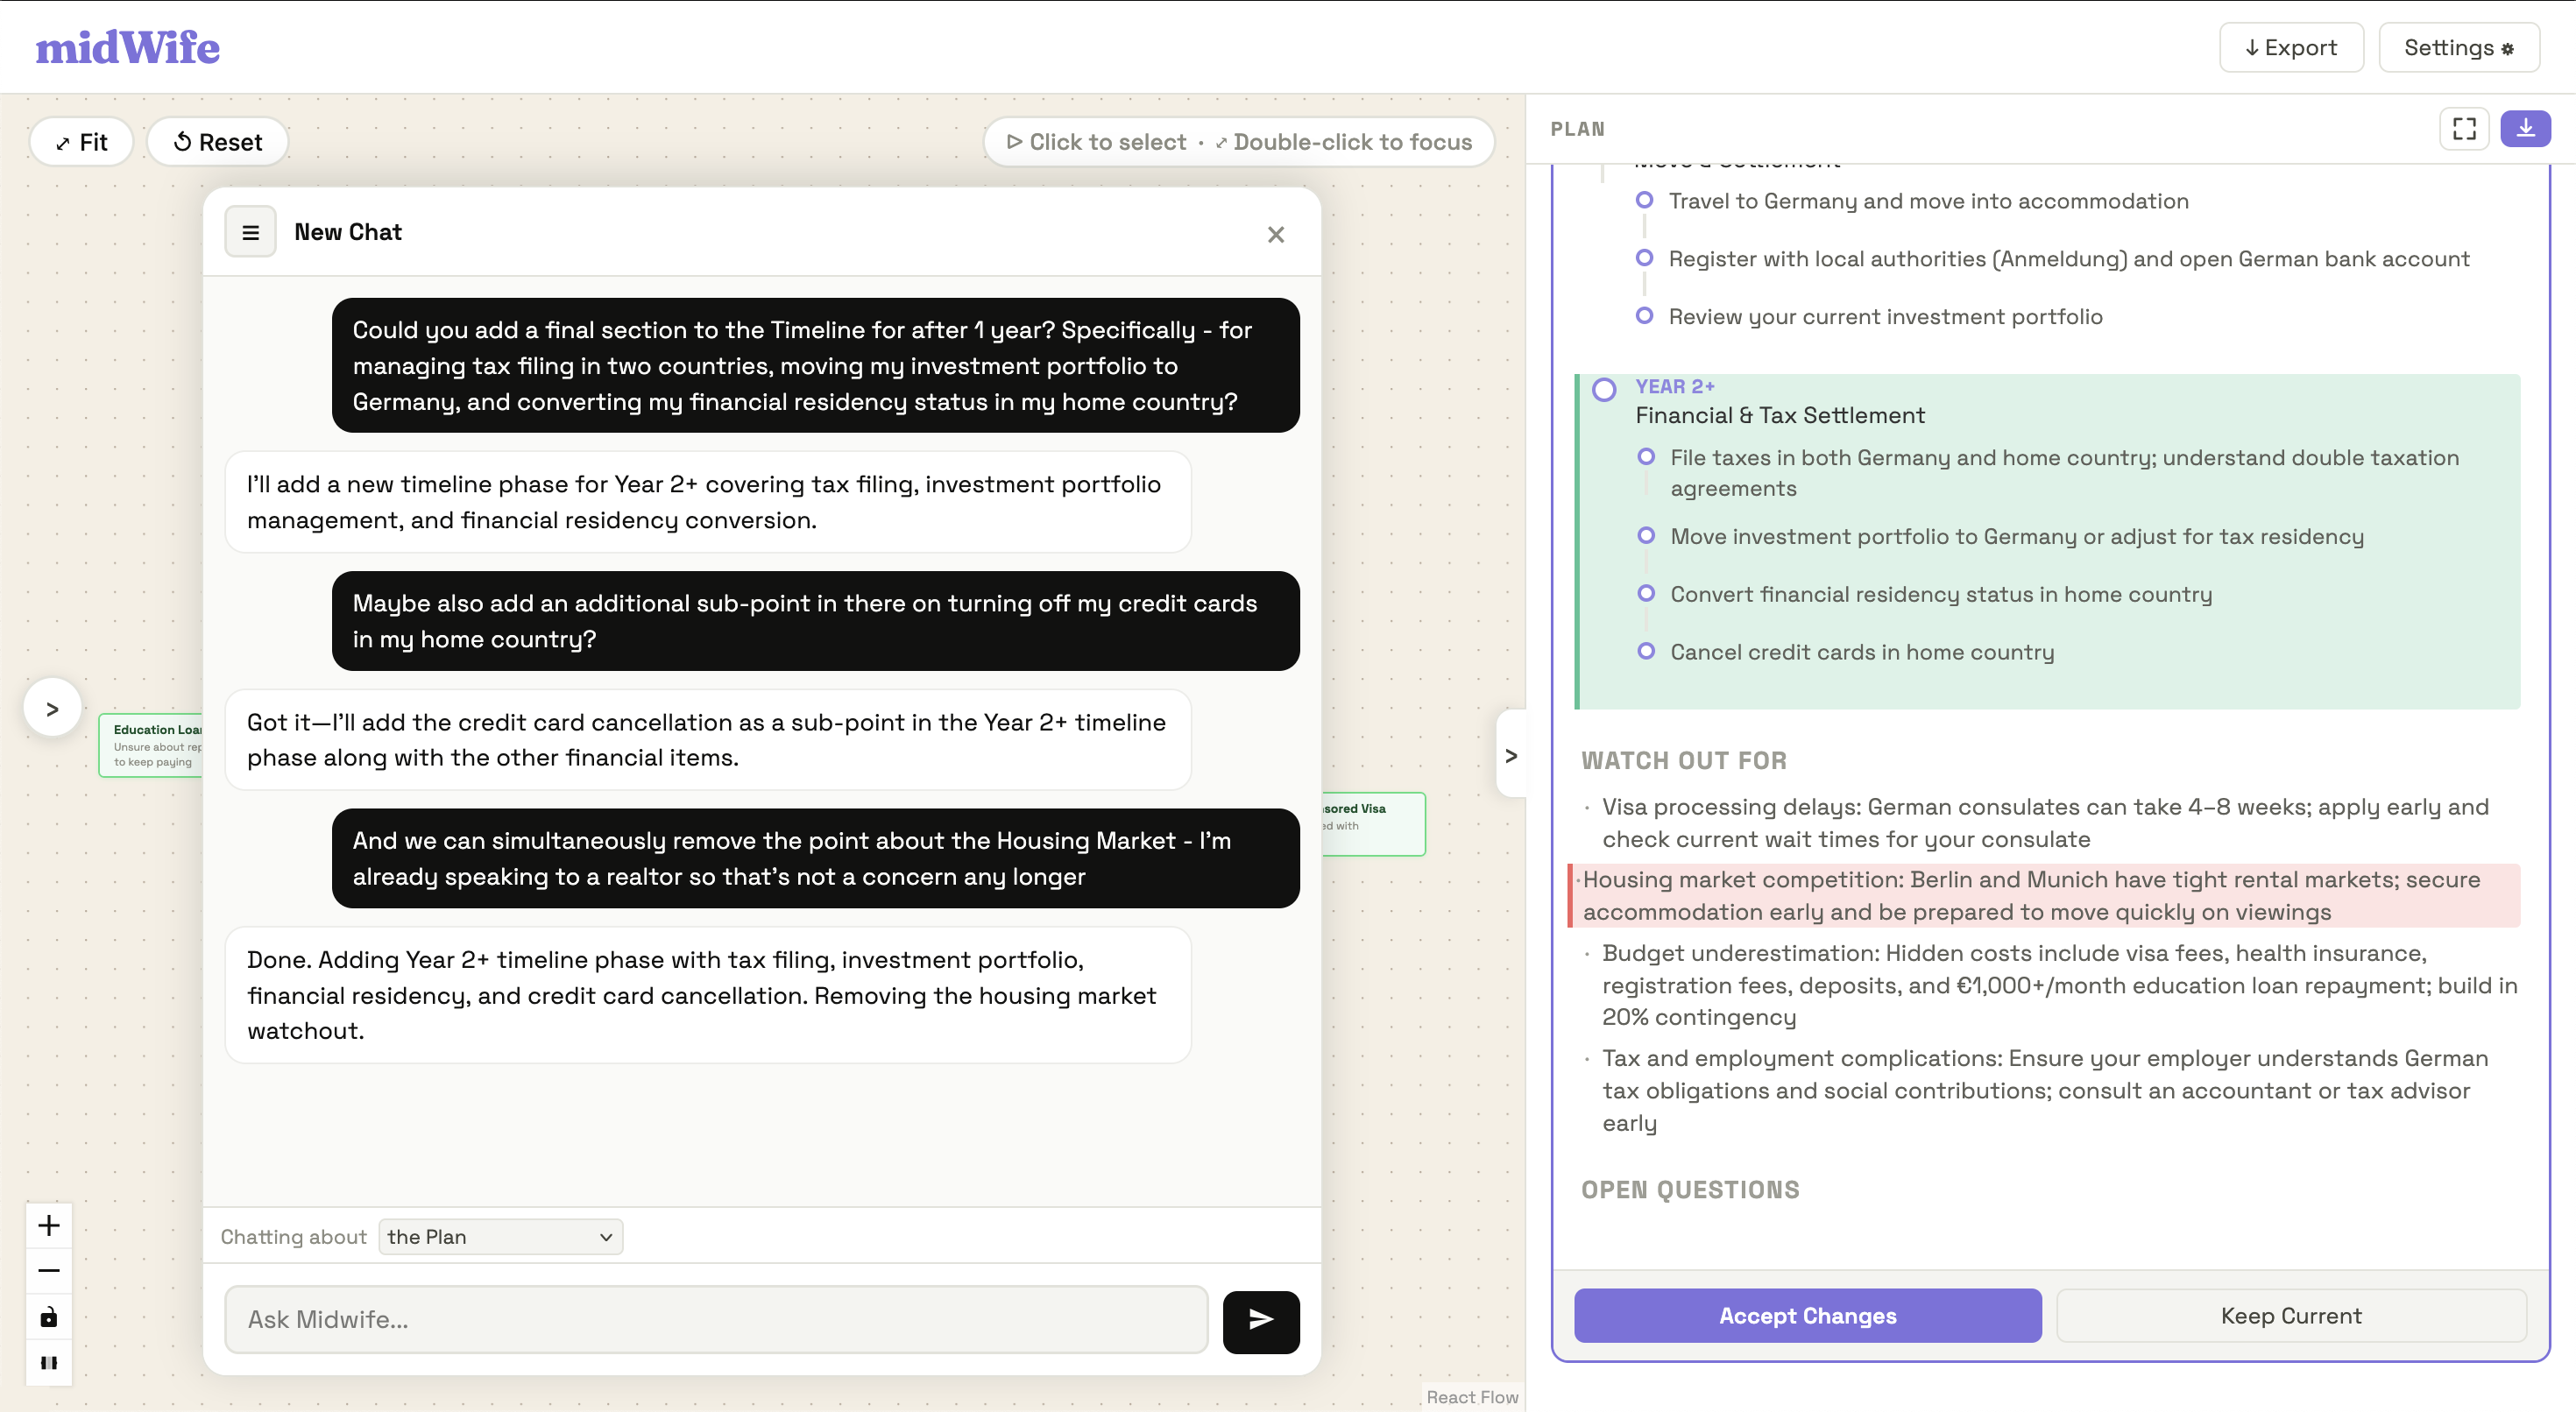
\includegraphics[width=\linewidth]{figures/usage}
  \caption{MidWife in use. (a) A planning session in progress: answered Aspect
  nodes (dark fill) branch into revealed children; the selected node's chat
  assistant is open. (b) The synthesis panel generated from the completed
  discourse, showing mode-specific tabs (Overview, Timeline, Tasks \& Resources,
  Open Questions).}
  \Description{Two-panel screenshot. Left panel shows the discourse canvas with
  a mix of answered and unanswered nodes and an open chat panel. Right panel
  shows the synthesis summary with four tabs of structured planning output.}
  \label{fig:usage}
\end{figure}

%%
%% After the figures, write 2–3 short paragraphs:
%%   Para 1: session management (UUID sessions, localStorage sync, up to 20
%%           resumable sessions, no server-side persistence required)
%%   Para 2: tree layout (ReactFlow + Dagre; left/right children based on edge
%%           sourceHandle; constants for ranksep/nodesep tuned for readability)
%%   Para 3: any noteworthy engineering decisions (e.g. the generate_aspects
%%           endpoint that lets users manually specify an aspect label and have
%%           the AI generate the Socratic question for it)
%%
midWife is built on a React + Vite frontend and a FastAPI backend (Figure~\ref{fig:architecture}).
The discourse canvas is implemented with ReactFlow, which provides native pan, zoom, and
node-selection at no interaction cost to the user. Tree layout is handled by Dagre, which
positions nodes automatically as the tree grows --- left and right children are assigned
based on edge source handle, ensuring the mindmap-style branching remains spatially
consistent regardless of tree depth or width. Layout constants (rank separation, node
separation) were tuned iteratively so that a fully elaborated tree with 20--30 nodes
remains readable without manual rearrangement.

The AI pipeline uses Claude Haiku 4.5 as the primary model, chosen for its low latency
and reliable structured-JSON output --- all Aspect labels, Socratic questions, and
suggestion chips arrive in a single round-trip, keeping the interview feel responsive.
A cascading Gemini fallback (2.0 Flash $\to$ 2.5 Flash $\to$ 3.1 Flash-lite) provides
graceful degradation under rate limits, transparent to the user. Three prompt engineering
decisions directly shape the interaction quality. First, \textit{covered\_aspects
deduplication}: all existing node labels are injected into each generation call as a
``do not repeat'' constraint, so users never encounter a duplicate or near-duplicate
Aspect as the tree grows. Second, \textit{context\_path injection}: the full ancestry
of label--question--answer triples is included in every elaboration prompt, causing
questions to grow progressively more specific with depth --- an effect users perceive
as the system tracking where they are in their thinking. Third, \textit{mode-specific
system prompts}: each of the nine planning modes installs a different questioning
persona and Aspect taxonomy (e.g.\ Research mode produces hypothesis, evidence, and
gap Aspects; Reflect mode produces introspective, first-person questions), so the same
tree interaction model feels meaningfully different across planning contexts. Finally,
when a user manually adds a node by specifying only a label, the backend's
\texttt{generate\_aspects} endpoint synthesises a Socratic question from that label and
its ancestry context, ensuring user-authored nodes are indistinguishable from
AI-generated ones in the interview flow.


%% ═══════════════════════════════════════════════════════════════════════════════
\section{Discussion}
%% ═══════════════════════════════════════════════════════════════════════════════
%%
%% TARGET: ~0.8 column.

%% ── 5.1 ───────────────────────────────────────────────────────────────────────
\subsection{Design Insights}
%%
%% Reflect on non-obvious things you learned building this. Suggested points:
%%
%%   Mode-awareness emerged from necessity: early testing showed that a
%%   single prompt style produced planning-flavoured questions even for
%%   reflection tasks. The 9-mode system was a direct response.
%%
%%   Ghost nodes as UX trade-off: prefetching makes elaboration feel instant,
%%   but ghost nodes are invisible to users, which creates a discoverability
%%   problem. The reveal interaction solves latency but obscures the AI's work.
%%
%%   Recontextualization is underused: the system can dynamically re-label
%%   ancestors as discourse deepens, but users rarely notice. This feature
%%   needs an affordance to surface proposed relabelings.
%%
%%   Per-node chat vs. global chat: anchoring the chat to a specific node's
%%   context was the single most important design decision for keeping
%%   conversations focused. A global chatbot would lose the discourse structure.
%%
%%   The synthesis panel as goal: users often don't know what "done" looks like
%%   in an open-ended planning session. The panel provides a concrete endpoint.
%%
TODO: Write design insights.

%% ── 5.2 ───────────────────────────────────────────────────────────────────────
\subsection{Limitations}
%%
%%   No user study: the current work is a design-and-build contribution.
%%   (This is consistent with the course project scope — explicitly noted.)
%%
%%   Ephemeral server sessions: the backend stores sessions in memory; a server
%%   restart clears them. localStorage preserves the tree structure but not
%%   all session metadata. Full persistence would require a database.
%%
%%   No tree export: users cannot export their discourse tree or summary panel
%%   to a document, slide deck, or task manager.
%%
%%   Mode-awareness is prompt-level only: modes change the AI's instructions
%%   but not the structural shape of the tree (e.g. logistics mode could
%%   generate a timeline-shaped subtree; it currently does not).
%%
%%   Recontextualization discoverability: see Design Insights above.
%%
TODO: Write limitations.

%% ── 5.3 ───────────────────────────────────────────────────────────────────────
\subsection{Future Evaluation}
%%
%% This directly addresses a grading criterion: "What would be the FIRST
%% element you would evaluate? Why?"
%%
%% Proposed first study:
%%   Design: within-subjects comparison of MidWife vs. ChatGPT for a
%%   structured planning task (e.g. planning a week-long trip, making a
%%   career decision).
%%
%%   Primary measure: decision coverage — the number of distinct planning
%%   dimensions addressed, rated by independent coders against a gold-standard
%%   checklist (method adapted from Sensecape [Suh 2023]).
%%
%%   Secondary measures: NASA-TLX (cognitive load), user-reported confidence
%%   in the final plan, perceived completeness, time-on-task.
%%
%%   Why this first: MidWife's central claim is that tree-structured Socratic
%%   dialogue surfaces more of the problem space than linear chat. Coverage is
%%   the most direct operationalisation of that claim, and a within-subjects
%%   design controls for individual differences in planning ability.
%%
%%   Prior art model: Sensecape [Suh 2023] used a similar within-subjects
%%   design with 12 participants; Luminate [Suh 2024] used 14 professionals.
%%   MidWife would need ~16–20 participants for adequate power.
%%
TODO: Write future evaluation subsection.

%% ── 5.4 ───────────────────────────────────────────────────────────────────────
\subsection{Future Directions}
%%
%%   Collaborative discourse trees: extend to multi-user sessions where
%%   teams co-construct a planning tree (CSCW angle; AMQuestioner explores
%%   this for argument maps [Pan 2025]).
%%
%%   Adaptive scaffolding: adjust Socratic question depth based on observed
%%   user behaviour (answer confidence, chat usage, elaboration rate) —
%%   operationalising Bhat et al.'s [2024] scaffolding-level findings.
%%
%%   Structured export: generate Markdown plans, Notion pages, or Gantt
%%   charts from the discourse tree, enabling the artifact to persist
%%   beyond the planning session.
%%
%%   Fine-tuned Socratic model: train a domain-specific model on dialogue
%%   trees to improve question quality, analogous to SocraticLM [Liu 2024].
%%
%%   Longitudinal deployment: study whether users return to completed trees,
%%   how trees evolve as plans change, and whether Socratic structure improves
%%   plan execution outcomes over weeks or months.
%%
TODO: Write future directions.


%% ═══════════════════════════════════════════════════════════════════════════════
\section{Conclusion}
%% ═══════════════════════════════════════════════════════════════════════════════
%%
%% TARGET: ~150 words.
%%
%% Restate: complex planning tasks outgrow linear chat. MidWife addresses this
%% by modelling deliberation as an interactive discourse tree in which an LLM
%% acts as a Socratic interlocutor. Key design contributions: mode-aware
%% questioning, mixed-initiative tree construction, per-node chat scoping,
%% and synthesis-as-endpoint. The prototype demonstrates the feasibility of
%% this paradigm; the natural next step is a controlled evaluation comparing
%% MidWife to standard LLM chat on structured planning tasks.
%%
TODO: Write conclusion.


%% ═══════════════════════════════════════════════════════════════════════════════
\begin{acks}
The author thanks Prof. Tovi Grossman and the CSC2524 seminar for the readings
and discussions that shaped this work.
\end{acks}

\bibliographystyle{ACM-Reference-Format}
\bibliography{midwife}

\end{document}
